\documentclass[11pt]{article}
\usepackage[a4paper,margin=21mm]{geometry}
\usepackage{amsmath,amssymb,booktabs,array}
\usepackage{tikz}
\usepackage[T1]{fontenc}
\usepackage{lmodern}
\usepackage[hidelinks]{hyperref}
\usepackage{listings}
\lstset{basicstyle=\ttfamily\small,breaklines=true,columns=fullflexible,frame=single}
\setlength{\parindent}{0pt}
\setlength{\parskip}{6pt}
\newcommand{\mos}[4]{\begin{scope}[shift={(#1,#2)}]
\draw (0,.24)--(0,-.24);
\draw (0,.20)--(.25,.20)--(.25,.5);
\draw (0,-.20)--(.25,-.20)--(.25,-.5);
\draw (-.16,.23)--(-.16,-.23);
\ifnum#4=1\draw (-.26,0) circle (.06);\draw (-.75,0)--(-.32,0);\else\draw (-.75,0)--(-.16,0);\fi
\node[anchor=east,font=\small] at (-.76,0) {$#3$};
\end{scope}}
\newcommand{\ground}[2]{\draw (#1,#2)--(#1,{#2-.12});\draw ({#1-.17},{#2-.12})--({#1+.17},{#2-.12});\draw ({#1-.11},{#2-.20})--({#1+.11},{#2-.20});}
\newcommand{\rail}[3]{\draw (#1,#2)--(#1,{#2+.15});\node[above,font=\small] at (#1,{#2+.15}) {$#3$};}
\newcommand{\outputnode}[3]{\fill (#1,#2) circle (.04);\draw (#1,#2)--({#1+.7},#2) node[right] {$#3$};}
\begin{document}
\begin{center}{\Large\bfseries Introduction to VLSI Design, 2020}\par{\large Homework 2: derivations, CMOS circuits, and code}\end{center}
The assignment itself is analytical. Runnable verification code and HSPICE decks are included to meet the requested programming deliverable. The local process model stays at \texttt{D:/cic018.l} and is not distributed.

\section*{1. Multi-$V_t$ design}
The circuit in Fig. 1 implements
\[
 D=\bar A\oplus B=AB+\bar A\bar B,\qquad E=\overline{BC}.
\]
In the given gate-delay abstraction, $A\to\text{INV}\to\text{XOR}\to D$ has delay 2; $B\to\text{XOR}\to D$ and $B/C\to\text{NAND}\to E$ have delay 1. Keep the D cone low-$V_t$. The E NAND has one unit of slack and can use high-$V_t$ devices \emph{provided its characterized total delay is at most 2 units}. Then the circuit's maximum delay remains 2 units while the NAND's subthreshold leakage decreases.

The problem does not give the high-$V_t$ delay or models, so preservation of timing is conditional on that bound. A physical guarantee for an arbitrary high-$V_t$ process would require characterized delays. Adding an inverter for $\bar B$ when implementing the XOR at transistor level adds a two-stage $B$ path; keep that inverter low-$V_t$ as well. The transistor schematic below implements D as XNOR directly using generated $\bar A,\bar B$.

\begin{center}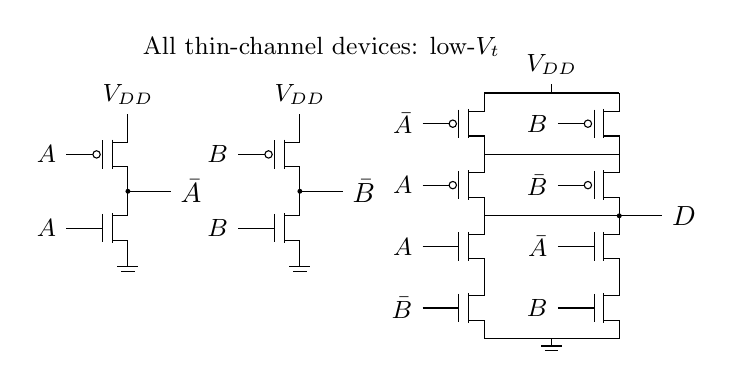
\begin{tikzpicture}[scale=.78]
% A/B complement inverters, all LVT
\mos{0}{2.5}{A}{1}\mos{0}{1.3}{A}{0}\draw (.25,1.8)--(.25,2);\outputnode{.25}{1.9}{\bar A}\rail{.25}{3}{V_{DD}}\ground{.25}{.8}
\mos{2.8}{2.5}{B}{1}\mos{2.8}{1.3}{B}{0}\draw (3.05,1.8)--(3.05,2);\outputnode{3.05}{1.9}{\bar B}\rail{3.05}{3}{V_{DD}}\ground{3.05}{.8}
% XNOR D complementary core
\mos{5.8}{3}{\bar A}{1}\mos{8}{3}{B}{1}
\mos{5.8}{2}{A}{1}\mos{8}{2}{\bar B}{1}
\draw (6.05,3.5)--(8.25,3.5);\rail{7.15}{3.5}{V_{DD}}\draw (6.05,2.5)--(8.25,2.5);
\draw (6.05,1.5)--(8.25,1.5);\outputnode{8.25}{1.5}{D}
\mos{5.8}{1}{A}{0}\mos{5.8}{0}{\bar B}{0}\mos{8}{1}{\bar A}{0}\mos{8}{0}{B}{0}
\draw (6.05,-.5)--(8.25,-.5);\ground{7.15}{-.5}
\node[font=\small] at (3.4,4.25){All thin-channel devices: low-$V_t$};
\end{tikzpicture}\qquad
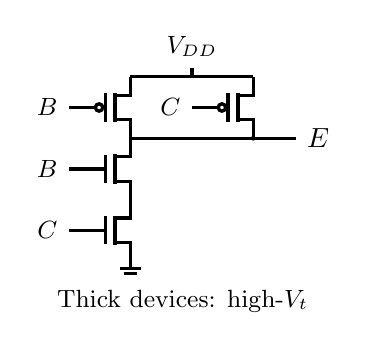
\begin{tikzpicture}[scale=.78]
\begin{scope}[very thick]
\mos{0}{2}{B}{1}\mos{2}{2}{C}{1}\draw (.25,2.5)--(2.25,2.5);\rail{1.25}{2.5}{V_{DD}}
\draw (.25,1.5)--(2.25,1.5);\outputnode{2.25}{1.5}{E}
\mos{0}{1}{B}{0}\mos{0}{0}{C}{0}\ground{.25}{-.5}
\end{scope}
\node[font=\small] at (1.1,-1.15){Thick devices: high-$V_t$};
\end{tikzpicture}\end{center}
The upper figure contains 12 low-$V_t$ devices; the E NAND contains 4 high-$V_t$ devices. \texttt{dualvt.sp} records this topology with explicit LVT/HVT model names. CIC018 TT supplies no separate characterized high-$V_t$ pair for this task; the file deliberately does not alias ordinary devices as high-$V_t$ devices.

\newpage
\section*{2. CMOS controlled rotator}
Exactly one of $c_0,c_1,c_2,c_3$ is 0 in the specified table. Write $s_k=\bar c_k$. Each output uses four parallel transmission gates, one selected by each $s_k$:
\begin{align*}
 z_0&=s_3a_0+s_2a_3+s_1a_2+s_0a_1,\\
 z_1&=s_3a_1+s_2a_0+s_1a_3+s_0a_2,\\
 z_2&=s_3a_2+s_2a_1+s_1a_0+s_0a_3,\\
 z_3&=s_3a_3+s_2a_2+s_1a_1+s_0a_0.
\end{align*}
Equivalently, for $c_k=0$, $z_j=a_{(j+k+1)\bmod4}$. This matches the original table in the order $c_3,c_2,c_1,c_0$.

\begin{center}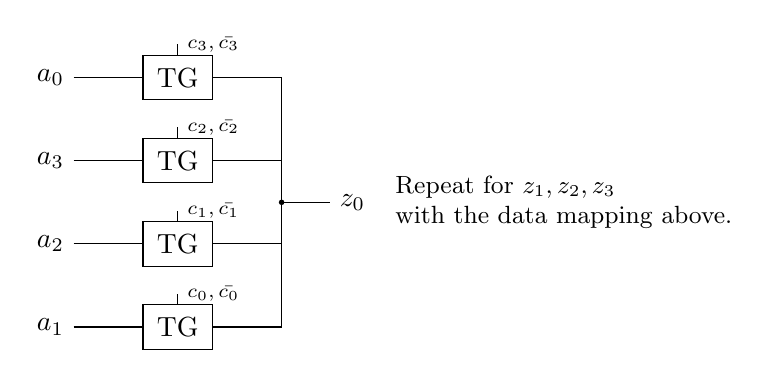
\begin{tikzpicture}[scale=.88]
% Four parallel transmission gate paths for z0
\foreach \y/\dat/\ctl in {0/a_1/c_0,1.2/a_2/c_1,2.4/a_3/c_2,3.6/a_0/c_3}{
\node[left] at (0,\y){$\dat$};\draw (0,\y)--(1,\y);
\draw (1,{\y-.32}) rectangle (2,{\y+.32});\node at (1.5,\y){TG};
\draw (2,\y)--(3,\y);\draw (1.5,{\y+.32})--(1.5,{\y+.48}) node[right,font=\scriptsize]{$\ctl,\bar{\ctl}$};}
\draw (3,0)--(3,3.6);\outputnode{3}{1.8}{z_0}
\node[align=left,font=\small,anchor=west] at (4.5,1.8){Repeat for $z_1,z_2,z_3$\\with the data mapping above.};
\end{tikzpicture}\end{center}

\textbf{Transistor-level TG and shared control inverter.} The PMOS gate uses $c_k$ and the NMOS gate uses $\bar c_k$. Both devices conduct when $c_k=0$, so either data rail passes without a threshold-voltage loss. PMOS bodies connect to $V_{DD}$, NMOS bodies to ground.
\begin{center}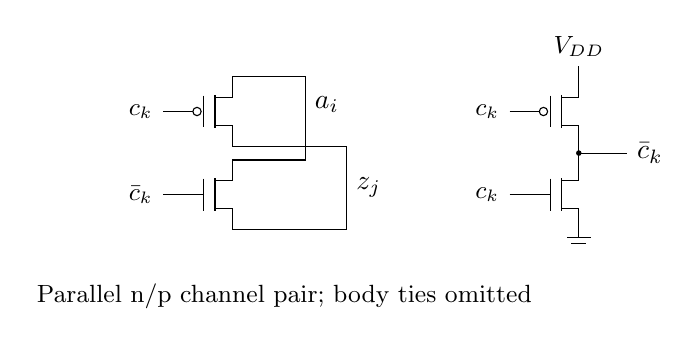
\begin{tikzpicture}[scale=.88]
\mos{0}{2}{c_k}{1}\mos{0}{.8}{\bar c_k}{0}
\draw (.25,2.5)--(1.3,2.5)--(1.3,1.3)--(.25,1.3);
\draw (.25,1.5)--(1.9,1.5)--(1.9,.3)--(.25,.3);
\node[right] at (1.9,.9){$z_j$};\draw (1.9,.9)--(1.9,.3);
\node[right] at (1.3,2.1){$a_i$};\draw (1.3,2.1)--(1.3,2.5);
\node[below,font=\small] at (1,-.35){Parallel n/p channel pair; body ties omitted};
\mos{5}{2}{c_k}{1}\mos{5}{.8}{c_k}{0}\draw (5.25,1.3)--(5.25,1.5);
\rail{5.25}{2.5}{V_{DD}}\ground{5.25}{.3}\outputnode{5.25}{1.4}{\bar c_k}
\end{tikzpicture}\end{center}
There are 16 TGs (32 MOSFETs) plus four shared control inverters (8 MOSFETs), for \textbf{40 transistors}. The supplied handwritten solution uses cascaded select paths; the direct one-hot arrangement is simpler and uses fewer devices. For invalid controls, multiple selected TGs can short unequal ideal data drivers or no TG can drive the output; the assignment specifies only the four valid control words. Control changes are sampled after settling.

\newpage
\section*{3. Pseudo-NMOS logic gate and sizing}
The PMOS is always on (gate tied to ground). The two NMOS devices are parallel. Thus the intended logic function is
\[
 \boxed{V_o=\overline{A+B}\quad\text{(a ratioed two-input NOR).}}
\]
Let $S_p=(W/L)_p$, $S_n=(W/L)_n$, and $r=S_n/S_p$ with equal NMOS sizes. For equal original sizes $R_p=2R_n$; scaling $W/L$ scales on-resistance inversely. Therefore
\[
 \frac{R'_p}{R'_n}=2r.
\]
For $AB=01$ or $10$, only one NMOS conducts; this is the worst low level:
\[
 \frac{V_{OL}}{V_{DD}}=\frac{R'_n}{R'_p+R'_n}=\frac{1}{2r+1}\le0.1
 \quad\Longrightarrow\quad\boxed{r\ge\frac92.}
\]
For $AB=11$, two NMOS resistances are in parallel, giving
\[
 \frac{V_o}{V_{DD}}=\frac{1}{4r+1}.
\]
For $AB=00$, the pull-down is off and $V_o=V_{DD}$. At $r=4.5$, the one-on cases are $0.1V_{DD}$ and the both-on case is $V_{DD}/19\approx0.05263V_{DD}$. A concrete minimum design is $L_p=L_n=0.18\,\mu$m, $W_p=0.5\,\mu$m and $W_{nA}=W_{nB}=2.25\,\mu$m. Choosing $W_n=2.5\,\mu$m ($r=5$) provides a small margin within the specified resistance model.

\begin{center}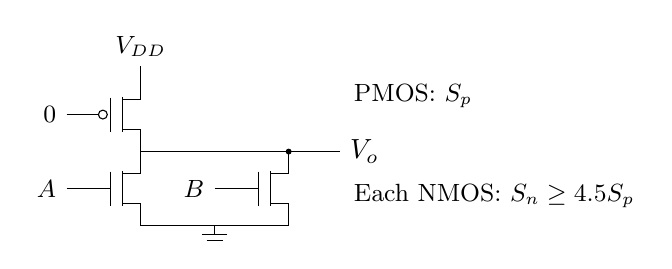
\begin{tikzpicture}[scale=.94]
\mos{0}{2}{0}{1}\rail{.25}{2.5}{V_{DD}}
\draw (.25,1.5)--(2.25,1.5);\outputnode{2.25}{1.5}{V_o}
\mos{0}{1}{A}{0}\mos{2}{1}{B}{0}\draw (.25,.5)--(2.25,.5);\ground{1.25}{.5}
\node[right,font=\small] at (3,2.25){PMOS: $S_p$};\node[right,font=\small] at (3,.9){Each NMOS: $S_n\ge4.5S_p$};
\end{tikzpicture}\end{center}
When the output is low, this ratioed gate consumes static current. In the ideal example $R_n=1\,\mathrm{k}\Omega$ for an original equal-size NMOS and $R_p=2\,\mathrm{k}\Omega$, the chosen $r=4.5$ gives $I_{01}=I_{10}=0.81$ mA and $I_{11}\approx0.8526$ mA at $V_{DD}=1.8$ V. Absolute resistance and current values are illustrative; the ratio bound is independent of that chosen resistance.

\section*{Reconciliation with the supplied answer}
The four-page \texttt{HW2\_answer.pdf}, by J.-M. Wu (107501503), correctly identifies XNOR/NAND, the rotator table, and NOR. Its first sizing derivation reverses the strength ratio and suggests $S_n/S_p=2/9$. The final handwritten correction obtains $9/2$ for one conducting NMOS and $9/4$ for two. The correct \emph{common design} is the stronger one-on constraint, $S_n/S_p\ge9/2$. The present solution retains that corrected result, makes the timing assumption explicit, and replaces the larger rotator with a shared-control 40T design.
\newpage\section*{Reproducible numerical evidence}
\texttt{python reproduce.py --model D:/cic018.l} generates the tables and decks and runs HSPICE. \texttt{--skip-hspice} runs the independent analytical checks only. The 64 valid rotator cases (16 data words for each of four controls) all passed in CIC018 TT at 1.8 V and 25 C with 1 fF on each output; highs were required to be at least 1.6 V and lows at most 0.2 V. The exported per-vector voltages are in \texttt{q2\_electrical.csv}.

The ideal-resistor HSPICE results exactly matched the separate closed-form calculation within $10^{-8}$ V. A supplementary nonlinear TT experiment was also run. These BSIM3 voltages are measured results for its declared sizes, not replacements for the assignment's fixed-resistance formula:
\begin{center}\begin{tabular}{r|rrrr}\toprule
$r$&$V_{00}$ (V)&$V_{01}$ (V)&$V_{10}$ (V)&$V_{11}$ (V)\\\midrule
1.0&1.800000&0.176482&0.176482&0.078389\\
4.5&1.800000&0.032241&0.032241&0.015732\\
5.0&1.800000&0.028826&0.028826&0.014100\\
\bottomrule\end{tabular}\end{center}
The measured supply currents are also saved in \texttt{q3\_cic018\_tt\_measurements.csv}. No electrical timing claim is made for Q1's unspecified high-$V_t$ models. \texttt{q1\_truth.csv} verifies all 8 input combinations and \texttt{q1\_timing.csv} states the gate-delay allocation and bound.

\end{document}
